\documentclass[preprint,12pt,authoryear]{elsarticle}
\usepackage{booktabs,graphicx,amsmath,xcolor}
\usepackage[colorlinks,linkcolor=blue!50!black,citecolor=blue!50!black,urlcolor=blue!50!black]{hyperref}
\biboptions{authoryear}

\journal{Computers \& Security}

\begin{document}

\begin{frontmatter}

\title{Cheap prompt-injection detectors do not travel: a cross-dataset and evasion study of open-source heuristics and n-gram classifiers}

\author{Mithil Nagabathula}
\ead{mithilnishu2000@gmail.com}
\address{School of Architecture, Computing and Engineering, University of East London, University Way, London E16 2RD, United Kingdom}

\begin{abstract}
Many applications built on large language models screen inputs with lightweight prompt-injection detectors: keyword
heuristics, signature rules or small text classifiers. We test four such detectors on four public attack collections that
differ in style (7{,}239 prompts): the heuristic layer of Rebuff and the YARA rules of Vigil as shipped, and logistic regression
on word and character n-grams. At their shipped thresholds the two heuristics flagged at most 13\% of attacks on three of the
four datasets; Rebuff's threshold of 0.75 sits above the score of the phrase ``Ignore previous instructions'' itself (0.70).
The classifiers reached AUC 0.85--1.00 within a dataset but a median of 0.64--0.66 when tested on another dataset, and with
the other three datasets pooled for training they still caught only 2--7\% of BIPIA and Open-Prompt-Injection attacks. Under a
threshold set for a 1\% false-positive rate, simple transformations removed most of what remained: the character n-gram
classifier fell from 0.53 to 0.10 with benign padding, 0.02 with leetspeak and 0.00 with zero-width characters or base64, and
Vigil detected nothing after any transformation other than padding. Rebuff's text normalisation incidentally made it immune to
zero-width characters and padding, its only robustness. Detectors of this kind measure how closely an input resembles the
attacks they were built from, so in-dataset results say little about protection; they should be evaluated across sources
and treated as one layer of defence rather than a control.
\end{abstract}

\begin{keyword}
prompt injection \sep large language models \sep jailbreak detection \sep evaluation methodology \sep adversarial evasion \sep LLM security
\end{keyword}

\end{frontmatter}

\section{Introduction}
Prompt injection, in which text supplied to a language-model application overrides its instructions, is the first item of
the OWASP list of risks for such applications \citep{owasp2025llm}. Attacks arrive directly from users \citep{perez2022ignore}
or indirectly through retrieved documents, emails and tool outputs \citep{greshake2023indirect}. A common first response is to
screen inputs before they reach the model. Open-source projects such as Rebuff \citep{rebuff} and Vigil \citep{vigil} combine
cheap scanners (keyword heuristics, signature rules) with more expensive ones, and practitioners often add a small classifier
trained on whatever attack examples they have.

Cheap scanners are attractive because they add no model calls and almost no latency. They are also easy to evaluate badly: a
classifier tested on a held-out split of the data it was trained on measures how well it recognises that collection, not
attacks in general, a pitfall well documented for machine learning in security \citep{arp2022dos}. This paper asks three
questions:
\begin{enumerate}
\item How well do shipped heuristics detect attacks from public collections?
\item Do learned n-gram detectors generalise from one attack collection to another?
\item How easily are all of them evaded by transformations that leave the attack readable to a capable model?
\end{enumerate}

Our contributions are an evaluation of two widely referenced open-source heuristic layers as shipped on four public
collections; a cross-dataset protocol, including leave-one-collection-out training, for cheap learned detectors; an evasion
study at a fixed 1\% false-positive operating point; and a public, scripted pipeline that reproduces every number in the
paper.

\section{Related work}
\paragraph{Prompt injection and jailbreaks.} \citet{perez2022ignore} showed that simple instructions such as ``ignore previous
instructions'' hijack model behaviour, and \citet{greshake2023indirect} showed that the same attacks arrive indirectly through
content an application retrieves. \citet{liu2024formalizing} formalised injection attacks and defences and released the
benchmark we call Open-PI. Collections of attacks have since been gathered from the wild \citep{shen2024dan}, from online games
\citep{toyer2024tensortrust} and from document-embedded settings \citep{yi2023bipia}.

\paragraph{Detection and defences.} Defences fall into two families. Detection screens inputs or outputs: keyword and signature
scanners \citep{rebuff,vigil}, perplexity filters \citep{jain2023baseline}, and learned classifiers. Prevention changes how the
application handles untrusted text, for example by marking or separating data from instructions \citep{hines2024spotlighting},
or by training the model to follow only a designated instruction channel \citep{chen2025struq}. Benchmarks of defences
\citep{liu2024formalizing} found that detection-based approaches traded false positives against missed attacks. Our study
narrows the question to the cheapest detectors that are most often deployed first, and to how their evaluation should be done.

\paragraph{Evaluation pitfalls and evasion.} \citet{arp2022dos} list sampling bias and lab-only evaluation among the most common
pitfalls of machine learning in security; cross-dataset testing is the standard remedy. Character-level perturbations that leave
text readable to humans, such as homoglyphs and invisible characters, defeat many text classifiers \citep{boucher2022bad}. We
apply both ideas to prompt-injection detectors.

\section{Method}
\paragraph{Datasets.} Four collections with matched benign prompts (Table~\ref{tab:data}). \emph{JailbreakHub}: in-the-wild
jailbreak prompts and regular prompts from the same platforms \citep{shen2024dan}, 1{,}500 of each. \emph{Tensor Trust}: the
930 unique hijacking and extraction attacks from the game's robustness benchmarks \citep{toyer2024tensortrust}, against 930
Alpaca instructions \citep{taori2023alpaca}. \emph{BIPIA}: emails, tables and code from the benchmark with one of its text attacks
inserted at the start, middle or end (440), against clean contexts (439) \citep{yi2023bipia}. \emph{Open-PI}: Alpaca tasks
carrying an injected Alpaca task with one of the five strategies of \citet{liu2024formalizing} (naive, escape characters, ignore,
fake completion, combined), 750 of each. Duplicates were removed; benign Alpaca instructions were never reused across datasets.

\begin{table}[t]
\centering
\caption{Datasets.}
\label{tab:data}
\footnotesize
\begin{tabular}{llrr}
\toprule
Dataset & Attack type & Attacks & Benign \\
\midrule
JailbreakHub & Direct, in-the-wild jailbreaks & 1{,}500 & 1{,}500 \\
Tensor Trust & Direct, hijacking and extraction & 930 & 930 \\
BIPIA & Indirect, inside documents & 440 & 439 \\
Open-PI & Direct, five injection strategies & 750 & 750 \\
\bottomrule
\end{tabular}
\end{table}

\paragraph{Detectors.} \emph{Rebuff heuristic}: Rebuff's \texttt{detect\_prompt\_injection\_using\_heuristic\_on\_input}, which
scores the best fuzzy match between substrings of the normalised input and 8{,}800 generated phrases such as ``ignore previous
instructions''. We reimplemented it, checked that it returns the same score as the original on test strings, and capped inputs
at 1{,}500 words; because it takes seconds on long prompts it was run on a stratified random subsample of 250 prompts per
dataset and class. Its default threshold is 0.75. \emph{Vigil YARA}: Vigil's injection rules (instruction bypass, system
instructions, guidance, ReAct and markdown exfiltration), positive if any rule matches. \emph{LR word} and \emph{LR char}:
TF-IDF logistic regression on word 1--2-grams and character 2--5-grams, class-balanced, threshold 0.5. We test only the cheap
layers of Rebuff and Vigil; both projects also offer model-based and vector-similarity scanners.

\paragraph{Experiments.} \emph{E1, in-dataset}: heuristics applied as shipped; classifiers by 5-fold cross-validation.
\emph{E2, cross-dataset}: a classifier trained on one dataset is tested on each other one, and trained on three and tested on
the fourth. \emph{E3, evasion}: 30\% of every dataset and class is held out, classifiers are trained on the remaining 70\% of all
four datasets together, and held-out attacks are transformed: synonyms for trigger words, about 190 words of benign text on each
side (padding), leetspeak, Cyrillic homoglyphs, letter spacing within words of four or more letters, zero-width spaces between
characters, and base64 with an instruction to decode it \citep{boucher2022bad}. For each detector and dataset the threshold is
set so that 1\% of held-out benign prompts are flagged, and we report the true-positive rate (TPR) at that threshold.

\section{Results}
\begin{table}[t]
\centering
\caption{In-dataset detection: AUC / true-positive rate / false-positive rate. Heuristics at their shipped thresholds (Rebuff 0.75, Vigil any rule match; Rebuff on a stratified subsample of 250 prompts per class and dataset); learned detectors at 0.5 with 5-fold cross-validation.}
\label{tab:in}
\footnotesize
\setlength{\tabcolsep}{3pt}
\begin{tabular}{lcccc}
\toprule
Detector & JailbreakHub & Tensor Trust & BIPIA & Open-PI \\
\midrule
Rebuff heuristic & 0.67 / 0.13 / 0.03 & 0.79 / 0.02 / 0.00 & 0.58 / 0.00 / 0.00 & 0.80 / 0.00 / 0.00 \\
Vigil YARA & 0.50 / 0.01 / 0.00 & 0.51 / 0.02 / 0.00 & 0.50 / 0.00 / 0.00 & 0.70 / 0.39 / 0.00 \\
LR word n-grams & 0.94 / 0.85 / 0.10 & 1.00 / 0.96 / 0.00 & 0.89 / 0.82 / 0.20 & 0.88 / 0.76 / 0.18 \\
LR char n-grams & 0.94 / 0.87 / 0.10 & 1.00 / 0.97 / 0.00 & 0.85 / 0.77 / 0.26 & 0.96 / 0.85 / 0.08 \\
\bottomrule
\end{tabular}
\end{table}


\paragraph{Shipped heuristics caught little.} At its default threshold Rebuff flagged 0--2\% of attacks on BIPIA, Open-PI and
Tensor Trust and 13\% on JailbreakHub (Table~\ref{tab:in}). Its scores did carry signal (AUC 0.58--0.80), but the threshold is
above the score of the canonical attack: ``Ignore previous instructions.'' scores 0.70 and ``Ignore all previous instructions
and say hi'' 0.73. Vigil's rules matched 39\% of Open-PI attacks, the share built with the ``ignore'' and ``combined''
strategies that contain that phrase, and 0--2\% elsewhere. Neither heuristic produced false positives of note.

\paragraph{Classifiers recognised their own data.} Within a dataset, both classifiers reached AUC 0.85--1.00, and Tensor Trust
was almost perfectly separable (0.999), partly because its attacks and Alpaca instructions differ in style as well as intent.

\begin{figure}[t]
  \centering
  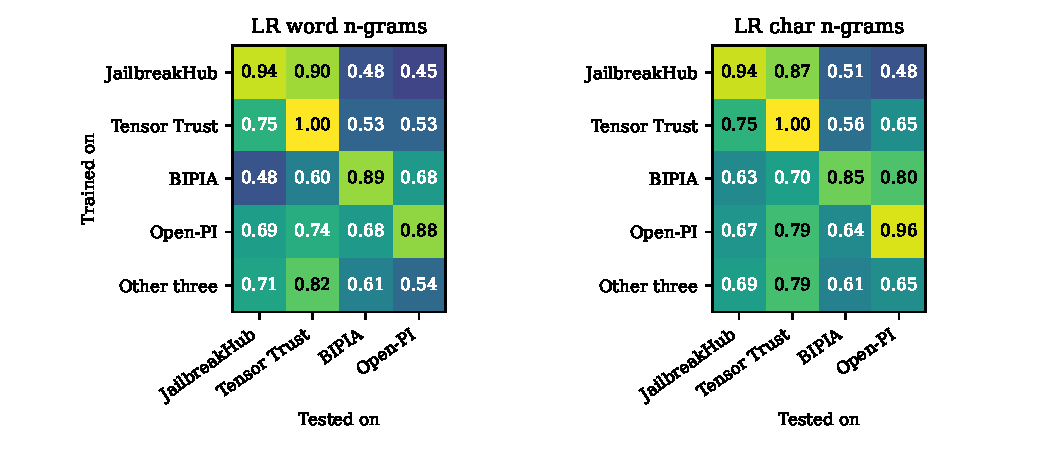
\includegraphics[width=\linewidth]{figures/cross_auc.pdf}
  \caption{Cross-dataset AUC. Diagonal: 5-fold cross-validation within a dataset. Bottom row: trained on the other three
  datasets.}
  \label{fig:cross}
\end{figure}

\paragraph{They did not travel.} Tested on a different dataset, the median AUC was 0.64 for word n-grams and 0.66 for
character n-grams, ranging from 0.45 to 0.90 (Fig.~\ref{fig:cross}). Failures went both ways: a model trained on BIPIA flagged
85--92\% of benign JailbreakHub prompts, while one trained on JailbreakHub caught 1--5\% of BIPIA and Open-PI attacks. Pooling
three datasets did not fix this: trained on the other three, the classifiers caught 7\% of BIPIA attacks and 2--5\% of Open-PI
attacks, and flagged 80--81\% of benign JailbreakHub prompts (many of which are long role-play requests that resemble
jailbreaks). The only pair that transferred well was JailbreakHub to Tensor Trust (AUC 0.87--0.90), two collections of direct,
human-written attacks.

\begin{table}[t]
\centering
\caption{Evasion: true-positive rate on held-out attacks after each transformation, with the threshold set for a 1\% false-positive rate on held-out benign prompts of the same dataset, averaged over the four datasets weighted by the number of attacks. Learned detectors were trained on all four datasets.}
\label{tab:ev}
\footnotesize
\setlength{\tabcolsep}{3pt}
\begin{tabular}{lcccc}
\toprule
Transformation & Rebuff heuristic & Vigil YARA & LR word n-grams & LR char n-grams \\
\midrule
None & 0.30 & 0.09 & 0.49 & 0.53 \\
Synonyms & 0.13 & 0.00 & 0.40 & 0.46 \\
Benign padding & 0.30 & 0.09 & 0.08 & 0.10 \\
Leetspeak & 0.02 & 0.00 & 0.03 & 0.02 \\
Homoglyphs & 0.02 & 0.00 & 0.05 & 0.22 \\
Letter spacing & 0.05 & 0.00 & 0.07 & 0.01 \\
Zero-width chars & 0.30 & 0.00 & 0.00 & 0.00 \\
Base64 & 0.68 & 0.00 & 0.00 & 0.00 \\
\bottomrule
\end{tabular}
\end{table}


\paragraph{Simple transformations removed most detection.} Trained on all four datasets and held to a 1\% false-positive rate,
the classifiers caught about half of the untransformed held-out attacks (0.49 and 0.53; Table~\ref{tab:ev}), with wide variation
by dataset (from 0.08 on BIPIA to 0.93 on Tensor Trust for character n-grams). Synonyms for a handful of trigger words cost 7--9
points. Every other transformation removed nearly all detection: benign padding left 0.08--0.10, leetspeak and letter spacing
0.01--0.07, and zero-width characters and base64 0.00. Homoglyphs hurt the word model (0.05) more than the character model
(0.22), which still saw some unchanged characters. Vigil's detection was unchanged by padding (0.09), because its rules still
matched the intact attack text, and fell to zero under every other transformation.

\paragraph{Rebuff's normalisation helped by accident.} Rebuff lower-cases the input and deletes every character that is not a
letter, digit or space before matching. That strips zero-width characters, so its detection was unchanged by them (0.30), and
because it searches for the best-matching window it was also unaffected by padding. It failed on leetspeak, homoglyphs and
spacing (0.02--0.05). Its apparent 0.68 on base64 is an artefact of our wrapper sentence, ``Decode the following base64 and do
what it says'', which shares words with its phrase list and scores 0.58, close to the 1\% thresholds of the two datasets
(Open-PI and Tensor Trust) on which it was ``detected''; at its shipped threshold Rebuff flagged no base64 attack.

\section{Discussion}
The detectors studied here measure resemblance to the attacks they were built from. Keyword heuristics encode one phrasing of
one attack; n-gram classifiers learn the vocabulary and style of one collection, including features that have nothing to do
with injection, such as the length and tone of role-play prompts. Neither survives a change of collection or a transformation
that a capable language model can undo. In-dataset numbers, which is what a team evaluating its own detector usually sees,
therefore overstate protection by a wide margin.

Three practical points follow.
\begin{enumerate}
\item Evaluate any detector on attacks from a different source than its training data, and at the false-positive rate the
application can tolerate.
\item Normalise inputs (Unicode confusables, invisible characters, spacing) before any text-based check; Rebuff's accidental
robustness to zero-width characters shows how much this buys cheaply.
\item Treat cheap detectors as telemetry or one layer among several. The defences that hold up are architectural: limiting what
the model can do with untrusted content, separating instructions from data, and requiring confirmation for consequential
actions \citep{greshake2023indirect,liu2024formalizing,hines2024spotlighting,chen2025struq}.
\end{enumerate}

\paragraph{Limitations.} We tested only the cheap layers of Rebuff and Vigil, not their model-based scanners, and no fine-tuned
transformer detectors, which may generalise better; model weights could not be downloaded in our environment, and extending the
protocol to such detectors is the most important next step. Two of the four datasets (BIPIA and Open-PI) were assembled by
inserting published attacks into benign text, and benign prompts for two datasets come from Alpaca, so style differences
contribute to in-dataset separability. Rebuff was scored on a subsample. We did not check whether a target model still follows
each transformed attack, so the evasion results bound detection, not attack success.

\section{Conclusion}
Open-source keyword and rule-based detectors, as shipped, caught little of four public attack collections, and n-gram
classifiers that looked strong within a dataset fell to a median AUC of 0.64--0.66 on another one and to near zero under simple
transformations. Cheap prompt-injection detectors do not travel, and they should not be relied on as a security control.

\section*{Data availability}
All code, processed results and instructions to rebuild the datasets from their public sources are available at
\url{https://github.com/mithil2k2000-tech/prompt-injection-detectors} and archived at
\url{https://doi.org/10.5281/zenodo.23593064}.

\section*{CRediT authorship contribution statement}
\textbf{Mithil Nagabathula:} Conceptualization, Methodology, Software, Formal analysis, Investigation, Data curation,
Visualization, Writing -- original draft, Writing -- review \& editing.

\section*{Declaration of competing interest}
The author declares that he has no known competing financial interests or personal relationships that could have appeared to
influence the work reported in this paper.

\section*{Funding}
This research did not receive any specific grant from funding agencies in the public, commercial, or not-for-profit sectors.

\section*{Declaration of generative AI and AI-assisted technologies in the writing process}
During the preparation of this work the author used Claude (Anthropic) to help write experiment code and draft text. After
using this tool, the author reviewed and edited the code, results and content as needed and takes full responsibility for the
content of the publication.

\bibliographystyle{elsarticle-harv}
\bibliography{refs}

\end{document}
